\chapter{Méthodologie}

\section{Travaux connexes}
\subsection{Classification supervisée de textes}
L'architecture classique pour la classification des textes provenant de descriptions des postes est composée d'une couche d'embedding à la tête d'une couche de convolution \endnote{\href{https://doi.org/10.1109/cispsse49931.2020.9212209}{Real-Time Resume Classification System Using LinkedIn Profile Descriptions}, S Ramraj and V. Sivakumar and Kaushik Ramnath G} ou de couches de récurrentes suivi d'une couche de convolution \endnote{\href{https://arxiv.org/pdf/1912.12214.pdf}{Job Prediction: From Deep Neural Network Models to Applications}, Tin Van Huynh and Kiet Van Nguyen and Ngan Luu-Thuy Nguyen and Anh Gia-Tuan Nguyen }. Entraînés uniquement sur les données textuelles sur les postes, les modèles performent très bien en atteignant des F1 de \textsf{72}.

L'architecture des transformers \endnote{\href{https://arxiv.org/abs/1706.03762}{Attention Is All You Need}, Ashish Vaswani and Noam Shazeer and Niki Parmar and Jakob Uszkoreit and Llion Jones and Aidan N. Gomez and Lukasz Kaiser and Illia Polosukhin} compile, après l'embedding, plusieurs couches d'encodeurs et de décodeurs composés de couches récurrentes. Le modèle est ensuite entraîné sur des phrases où des mots sont masqués, et sur des textes où des phrases sont à deviner.

\subsection{Données déséquilibrées}
L'algorithme SMOTE \endnote{\href{https://arxiv.org/pdf/1106.1813.pdf}{SMOTE: Synthetic Minority over-Sampling Technique}, Chawla, Nitesh V. and Bowyer, Kevin W. and Hall, Lawrence O. and Kegelmeyer, W. Philip} est l'outil classique pour gérer les données déséquilibrées en effectuant un sous-échantillonnage des classes dominantes et un sur-échantillonnage des classes sous-représentées en s'aidant des méthodes à noyau. Cet algorithme ne peut s'employer que sur une représentation tabulaire des textes (TF-IDF, occurences, ...) mais ne tient pas compte du contexte. La version WEMOTE \endnote{\href{https://www.sentic.net/wisdom2014chen.pdf}{WEMOTE - Word Embedding based Minority Oversampling Technique for Imbalanced Emotion and Sentiment Classification}, Tao Chen and Qin Lu and R. Xu and Bin Liu and J. Xu} applicable sur les embeddings effectue le sur-échantillonnage en prenant en compte la représentation du texte mais ne permet pas encore de faire de meilleures performances par rapport à SMOTE.

Les travaux sur la correction des biais basés sur le genre dans le traitement de language naturel \endnote{\href{https://www.aclweb.org/anthology/P19-1159}{Mitigating Gender Bias in Natural Language Processing: Literature Review}, Sun, Tony  and Gaut and al.} ont démontré que les corrections de logits après les prédictions permettent de réduire le biais certes mais réduisent beaucoup trop les performances. Les solutions en amont sont: la suppression de l'axe du genre dans les embeddings \endnote{Gender Bias in Contextualized Word Embeddings, Jieyu Zhao and Tianlu Wang and Mark Yatskar and Ryan Cotterell and Vicente Ordonez and Kai-Wei Chang} si elle est détectée, l'augmentation des données \endnote{\href{https://www.aclweb.org/anthology/D19-5543}{Improving Neural Machine Translation Robustness via Data Augmentation: Beyond Back-Translation}, Li, Zhenhao  and Specia, Lucia} accompagnée ou non de l'inter-changement des genres en utilisant de la reconnaissance d'entité nommée (NER) pour les noms et les postes, ainsi que l'inversement des genres des mots en s'aidant de l'étiquetage morpho-syntaxique (PosTag).

\subsection{Nettoyage des labels}
L'algorithme t-SNE \endnote{\href{https://jmlr.org/papers/volume9/vandermaaten08a/vandermaaten08a.pdf}{Visualizing Data using t-SNE}, Geoffrey Hinton and Laurens van der Maaten} permet de visualiser la proximité et la disparité des labels. La représentation des données permet ensuite de visualiser la distribution des labels sur les deux axes principales. L'algorithme WAR \endnote{\href{https://arxiv.org/pdf/1904.03936.pdf}{Wasserstein Adversarial Regularization (WAR) on label noise}, Bharath Bhushan Damodaran and Kilian Fatras and Sylvain Lobry and Rémi Flamary and Devis Tuia and Nicolas Courty} permet une régularisation des données en séparant les labels en utilisant la distance de Wasserstein.


\section{Travaux effectués}
\subsection{Pré-traitements}
\subsubsection{Nettoyage des labels}
\hfill\\
En examinant les données, nous avons relevé des descriptions ambiguës pour un même label. Il s'agit du poste "\textit{architect}" qui comprend des descriptions pour les architectes en constructions et les architectes informatiques. Le premier étant proche du label "\textit{interior designer}", alors que le second se rapproche plus de "\textit{software engineer}".


\begin{longtable}{l p{4in}}
    &\\
    \textit{architect}: &"He runs a boutique design studio attending clients. His work explores the convergence of human arts and science to give shape to an ever evolving design practice." \\
    &\\
    \textit{architect}: &"He focuses on cloud security, identity and access management, mobility security, and security for Microsoft platforms and solutions."\\
    &
\end{longtable}

Pour séparer le label, nous avons opté pour le modèle de l'Allocation de Dirichlet latente (LDA) où le but est d'effectuer un clustering en regroupant les données de ce label par leur sujet, c'est-à-dire la fréquence des mots utilisés. Nous avons choisi la log-vraisemblance pour mesurer la qualité de nos clusters, en cherchant par GridSearchCV les paramètres optimaux pour le nombre de clusters et le learning decay. Nous avons gardé \textsf{2} clusters et un learning decay de \textsf{0.5} pour le label "\textit{architect}", et avons donc ajouté le label 29 aux catégories pour "\textit{data architect}".\\
L'opération étant assez coûteuse et n'ayant pas observé plus d'ambiguïtés pour le reste des labels, nous n'avons pas étendu le nettoyage des labels sur l'ensemble des données.

\hfill\\
\subsubsection{Augmentation de donnée}
\hfill\\
Lors de ces travaux, nous avons traité le problème du biais sur le genre comme un problème de données déséquilibrées. En effet, les données sur un poste stéréotypé pour un genre sous représente l'autre genre, et crée donc un déséquilibre par rapport à la mesure sur cette variable.

Nous n'avons pas choisi les algorithmes SMOTE, WEMOTE et la suppression de l'axe du genre dans les embeddings; ces solutions étant dépendantes de la représentation du corpus. Nous avons opté pour la Beyond-Back Translation \endnote{\href{https://www.aclweb.org/anthology/D19-5543}{Improving Neural Machine Translation Robustness via Data Augmentation: Beyond Back-Translation}, Li, Zhenhao  and Specia, Lucia} qui consiste à créer des nuances de mots et de syntaxe en s'appuyant sur les différences d'expressions entre les langues.

La deuxième méthode est l'inversement du genre (GenderSwap\endnote{\href{https://www.aclweb.org/anthology/N18-2003}{Gender Bias in Coreference Resolution: Evaluation and Debiasing Methods}, Zhao, Jieyu  and Wang, Tianlu  and Yatskar, Mark  and Ordonez, Vicente  and Chang, Kai-Wei} \endnote{\href{https://github.com/valleyviolet/gender_swap}{Gender Swap}, https://github.com/valleyviolet}). Cependant, nous n'avons pas utilisé les techniques habituelles avec la NER et les PosTag, mais plutôt des embeddings de Word2vec en appliquant à l'échelle d'une phrase l'opération vectorielle dont l'exemple classique est \texttt{king - male + female = queen}.
\\
Pour sur-échantillonner le genre sous-représenté pour un label nous avons sélectionné au hasard la moitié des données du genre ainsi que le quart du genre opposé. Les traductions ont été faites en \texttt{Anglais - Français - Anglais} sur cet échantillon et le GenderSwaping a été appliqué sur les données provenant du quart du genre opposé.

\begin{longtable}{l p{4in}}
    &\\
    \textbf{original}: &"Jane is the pastor's wife and she gets up every morning to light the candles in the church." \\
    &\\
    \textbf{beyond back}: &"Jane is the priest's spouse and she wakes up every morning to light the candles of the chapel."\\
    &\\
    \textbf{gender swap}: &"John is the husband of the priestess and he wakes up every morning to light the candles of the chapel."\\
    &
\end{longtable}


\subsection{Modèles de classification}
\subsubsection{Support Vector Machine Linéaire}
\hfill\\
Pour les modèles classiques, nous avons opté pour la représentation TF-IDF du corpus, en sélectionnant ensuite les \textsf{133 000}\sidenote{limite imposée par nos machines} meilleurs variables par un test de chi2.

Nous avons donc effectué un benchmark naïf sur les modèles classiques de classifications et nous avons observé \texttt{Linear SVC} et \texttt{Ridge Classifier} se démarquer. Ces deux modèles ont donc été optimisés chacun par la méthode \textit{Nested GridSearchCV} sur \textsf{5} folds internes et \textsf{3} folds externes. Le modèle du machine à vecteur support est celui qui a le mieux performé en terme de F1-score et de Disparate Impact. Toutefois, le modèle tel quel ne produit pas de logits à la prédiction, nécessaire aux méthodes d'ensembles qu'on envisage pour la suite.\\
La méthode \texttt{Calibrated CV} donne les probabilités d'obtenir à une classe dans un problème à multi-classe en utilisant une méthode d'ensemble sur un estimateur de base déjà entraîné. Cette calibration a légèrement amélioré les performances de \texttt{Linear SVC} lors de la phase de test.

\hfill\\
\subsubsection{Roberta}
\hfill\\

Le modèle \endnote{\href{https://arxiv.org/pdf/1907.11692.pdf}{RoBERTa}, Yinhan Liu et al. 2019} est un modèle de transformer basé sur BERT. L'architecture est la même, mais certains changements sur le prétraitement des données sont appliquées, comme le masquage dynamique, une taille de batch plus importante, et un encodage BPE plus large. Aussi, ce modèle est entrainé avec plus de passes, et sur un corpus plus important. \\
De manière générale, RoBERTa (ou d'autres transformers), après quelques epochs de fine-tuning, permettent d'arriver à un F1-score beaucoup plus grand, et surtout ces modèles (surtout ls plus larges avec 300M ou plus paramètres) semblent moins sensible au déséquilibre des classes cibles. Cependant, comme nous le présentons plus en détail plus loin, quelques problèmes d'instabilité commencent à apparaitre sur ces gros modèles.

\hfill\\
\subsubsection{Electra}
\hfill\\

\hfill\\
\subsubsection{Le modèle générateur T5}
\hfill\\
Le modèle T5 est un modèle de transformer encoder-decoder créé par GoogleAI\endnote{\href{https://arxiv.org/abs/1910.10683}{Exploring the Limits of Transfer Learning with a Unified Text-to-Text Transformer}, Colin Raffel and Noam Shazeer and Adam Roberts and Katherine Lee and Sharan Narang and Michael Matena and Yanqi Zhou and Wei Li and Peter J. Liu} dont le but est d'unifier toutes les tâches de NLP. La motivation principale réside dans le fait que tous les problèmes de NLP peuvent être transformé en problème de Text-to-Text.

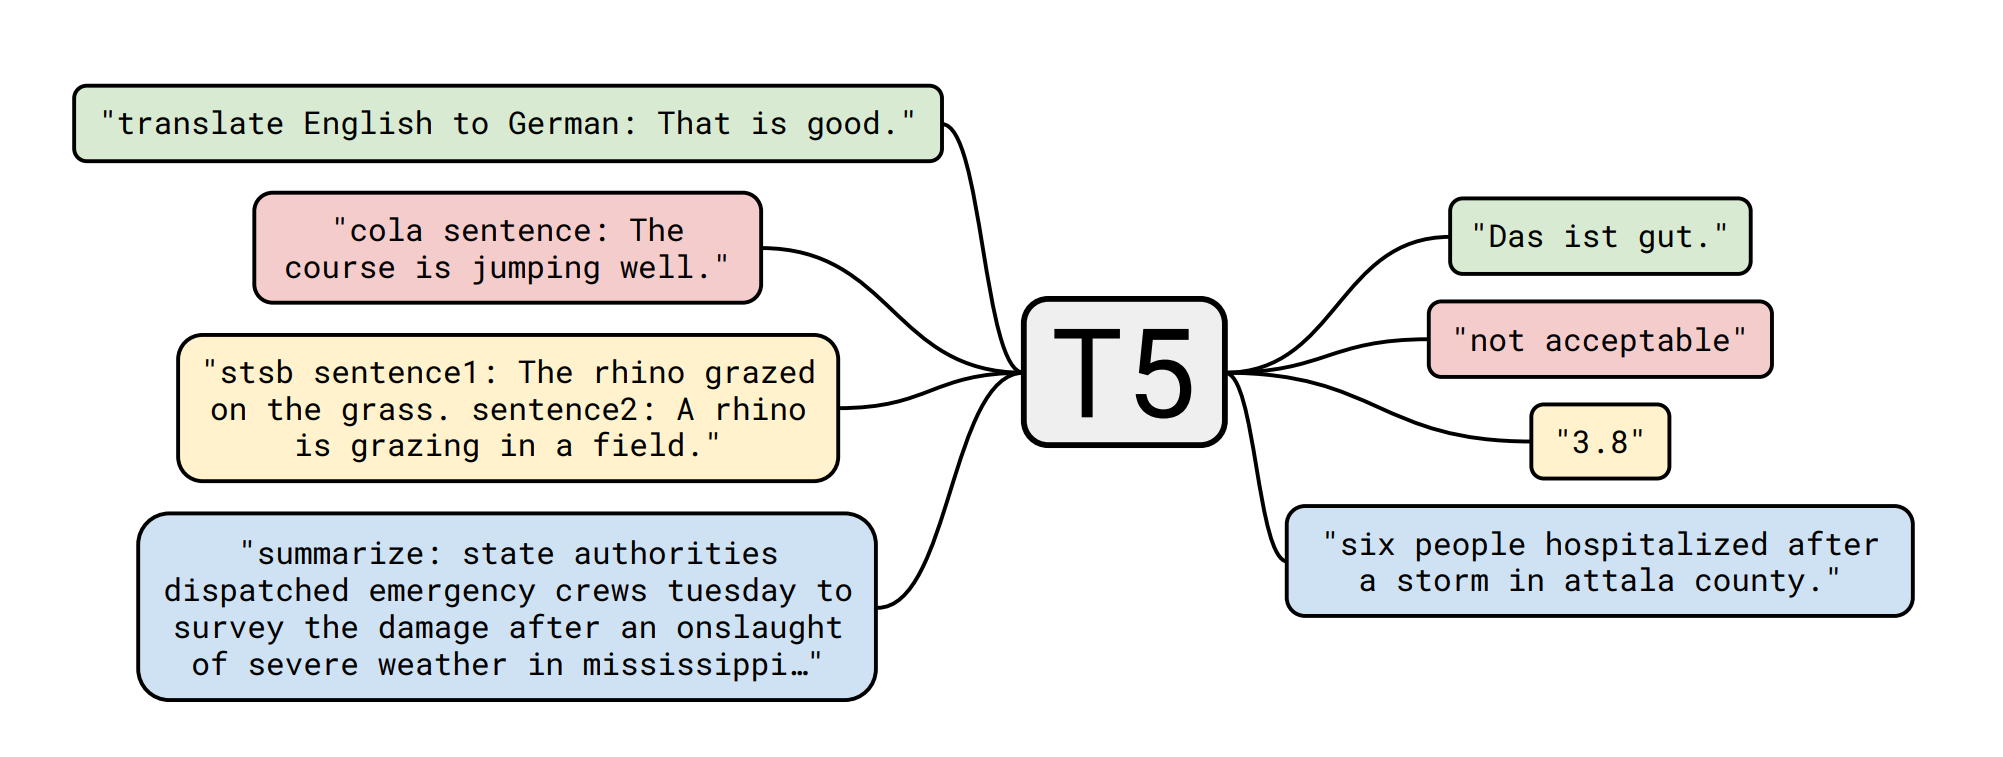
\includegraphics[width=\textwidth]{t5googleai.png}

Dans notre cas, l'encoder reçoit la description, une séquence d'environ 190 tokens, et le décode en nom de poste, soit un séquence de 4 tokens pour notre problème. L'avantage par rapport aux modèles de classification précédents réside dans le fait que le modèle obtient aussi des informations provenant de la représentation du label lors de l'entraînement, au lieu d'un unique chiffre.
Le revers, c'est l'espace de génération du modèle qui s'étend théoriquement sur tous les mots de la langue anglaise, ce qui donne des labels qui n'existent pas dans nos données mais qui s'en rapprochent.\\
Nous avions par exemples, pour "\textit{yoga teacher}", les dénominations "\textit{pilates coach}" et "\textit{meditation teacher}". Pour re-calibrer les données, les scores de similarités basés sur les synonymes avec \texttt{wordnet} aux labels sont calculés sur les sorties générées. Dans notre cas, les labels sont assez disparates et les différentes dénominations des sorties sont rares.

\hfill\\
\subsubsection{La méthode d'ensemble}
\hfill\\

Lors de nos premiers essais avec des architectures transformers, qui était avec des petits modèles, de l'ordre d'une cinquantaine de millions de paramètres, rien n'était à signaler, les résultats était stables d'un essai à l'autre, même avec exactement les mêmes hyper-paramètres. Ce n'est que lorsque nous commençons à utiliser des modèles pré-entrainés beaucoup plus large (quelques centaine de millions paramètres) que les résultats deviennent moins stables. Tout d'abord de temps à autre, durant certains tests, la perte d'entrainement se mettait à remonter d'un coup, avec l'accuracy pouvant passer de 80\% à presque 0 en quelques batchs seulement. Une autre instabilité survient dans les résultats, les différences dans le macro f1-score estimé deviennent beaucoup plus grande, entre 0.80 et 0.83. \\

L'une des ressources les plus utile pour cette compétition à été les précédentes compétitions de traitement du language sur Kaggle, notamment \href{https://www.kaggle.com/c/jigsaw-multilingual-toxic-comment-classification/overview}{Jigsaw Multilingual Toxic Comment Classification} et les discussions et présentations des différents membres du top10. Surtout, c'est en lisant les solution de l'équipe gagnante que nous en sommes venu à tester les techniques présentées dans ce chapitre \endnote{\href{https://www.kaggle.com/c/jigsaw-multilingual-toxic-comment-classification/discussion/160862}{1st place solution overview}, Chun Ming Lee et rafiko1}. Cette équipe présente notamment deux articles traitant de l'instabilité des transformers, le premier s'interessant à l'impact de l'initialisation des poids de la dernière couche (de classification) \endnote{\href{https://arxiv.org/pdf/2002.06305.pdf}{Fine-Tuning Pretrained Language Models: Weight Initializations, Data Orders, and Early Stopping}, J. Dodge et al. 2020}, le deuxième essayant de traiter le problème via du bagging \endnote{\href{https://www.aclweb.org/anthology/2020.trac-1.9.pdf}{Bagging BERT Models for Robust Aggression Identification}, Julian Risch and Ralf Krestel 2020}. Par manque de temps, mais aussi puisque la solution du premier article apporte de bon résultats, nous n'avons pas tester le bagging de transformers. \\
Dans cet article, les tests sont fait en monitorant en continu la qualité des graines, c'est à dire en laissant un échantillon de coté. Puis ils choisissent de prendre un ensemble (soft voting) des dix meilleures graines parmi trente. Cependant pour nous, cela n'est pas forcément satisfaisant, car nous n'avons pas envie de nous séparer d'un partie des données. En effet, pour repérer les "bonnes" graines, nous aurions besoin d'un échantillon de validation, car les bonnes graines dépendent des données. \\
Nous choisissons plutôt d'expérimenter avec un protocole que nous pourrions répéter sur l'échantillon d'apprentissage en entier dans le cas où les résultats sont concluant. Plutôt que de choisir des graines, nous essayons de voir si le fait de prendre l'ensemble de plusieurs graines au hasard, est meilleur  qu'une graine toute seule prise au hasard. Ainsi, notre classifier devient : $$ \hat y = \argmax_j \sum_{i=1}^n p_{i,j} $$ où $p_{i,j}$ est la probabilité pour la classe $j$ prédite par le $i$-ème classifier (parmi $n$ graines/classifiers). \\

Une autre méthode pour essayer de stabiliser les résultats survient durant l'entrainement, plutôt que de choisir une epoch optimale via un echantillon de validation, en surveillant la val-loss, il est possible de faire un prédiction après chaque epoch, et de faire un ensemble de toutes les prédictions (via un soft-voting de nouveau), le résultats en terme de F1-score est bluffant. Sur le graphique si dessus, les série de couleur claires sont les scores des prédictions unique après chaque epoch, les séries de couleur foncées sont les scores de l'ensemble des prédictions des epoch, allant de la 1ère à la i-ème.

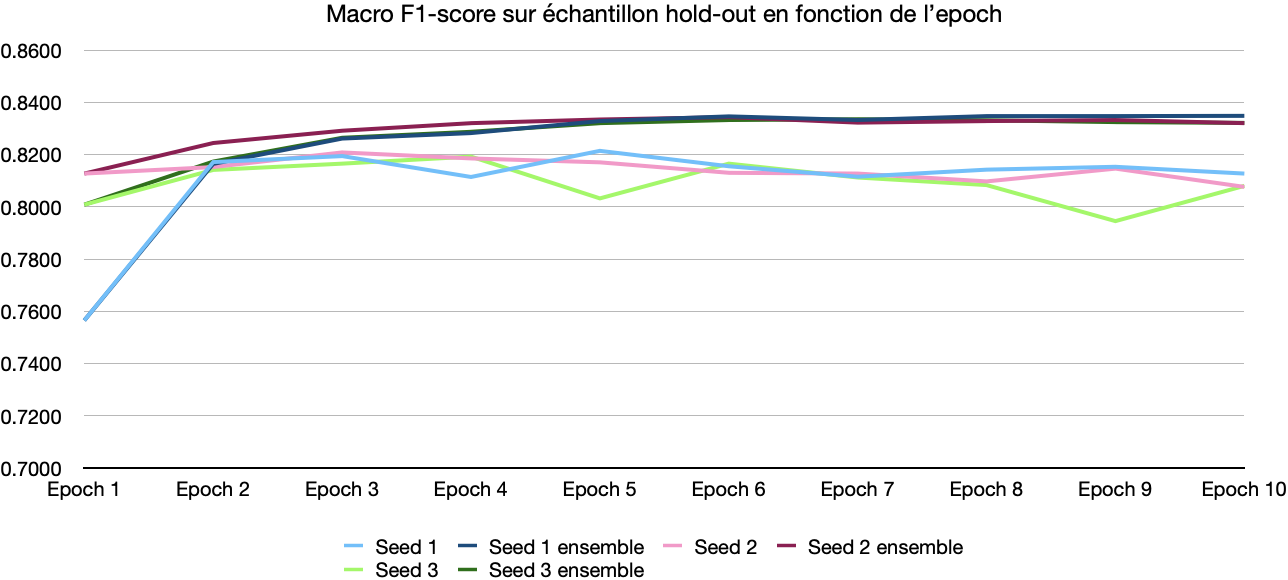
\includegraphics[width=\textwidth]{Untitled.png}

Finalement, en prenant ces deux méthodes en même temps, notre ensemble peut-être vu de la façon suivante :
$$ \hat y = \argmax_j \sum_{i=1}^n p_{i,j,e} $$ où $p_{i,j,e}$ est la probabilité pour la classe $j$ prédite par le $i$-ème classifier (parmi $n$ graines/classifiers) et à la $e$-ème epoch.

%%% Local Variables: 
%%% mode: latex
%%% TeX-master: master
%%% End: 